\chapter{PAPER 4 TITLE GOES HERE}
% \label{polymer_fibers1}

\begin{center}
    Authors and Affiliations %\\
    \blfootnote{Modified from a manuscript to be submitted to/ under review/ published in \textit{Name of the Journal}}
\end{center}

\section{Abstract}
This is the text of my abstract that is part of the thesis itself.
The abstract describes the work in the first paper general. You can use the same abstract as your paper here.

%\pagebreak %remove if needed

% Please include sections as the paper has, some of the following sections are meant as examples of what can be done, the bibliography should be made as given
%\section{Overview}

This is the opening paragraph to my thesis which
explains in general terms the concepts and hypothesis
which will be used in my thesis.

With more general information given here than really
necessary.

\section{Introduction}

Here initial concepts and conditions are explained and
several hypothesis are mentioned in brief.

Of course, data on this as seen in Table~\ref{data}
is few and far between.

\begin{table}[h!tb] \centering
\isucaption{Moon Data}
\label{data}
% Use: \begin{tabular{|lcc|} to put table in a box
\tagpdfsetup{table/header-rows={1}}
\begin{tabular}{lcc} \hline
\textbf{Element} & \textbf{Control} & \textbf{Experimental} \\ \hline
Moon Rings & 1.23 & 3.38 \\
Moon Tides & 2.26 & 3.12 \\
Moon Walk & 3.33 & 9.29 \\ \hline
\end{tabular}
\end{table}


\subsection{Hypothesis}

Here one particular hypothesis is explained in depth
and is examined in the light of current literature.

Or graphically as seen in Figure~\ref{mgraph}
it is certain that my hypothesis is true.

\begin{figure}[h!tb] \centering

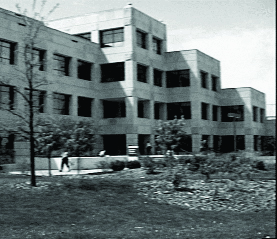
\includegraphics[alt={Here is some alt text}]{Images/dc5}

\isucaption{Durham Centre}
\label{mgraph}
\end{figure}

\subsubsection{Parts of the hypothesis}

Here one particular part of the hypothesis that is 
currently being explained is examined and particular
elements of that part are given careful scrutiny.

% Below \subsubsection
% Sectional commands: \paragraph and \subparagraph may also be used

\subsection{Second Hypothesis}

Here one particular hypothesis is explained in depth
and is examined in the light of current literature.

\subsubsection{Parts of the second hypothesis}

Here one particular part of the hypothesis that is 
currently being explained is examined and particular
elements of that part are given careful scrutiny.

\section{Criteria Review}

Here certain criteria are explained thus eventually
leading to a foregone conclusion.

\section{Results}

\section{Conclusion}\label{conclusion3}

The conclusion of the paper goes here.

%%%%
% Reference section comes before the appendix

%\bibliographystyle{acm} % use for numbered citations along with options given in preamble. Look at the main thesis.tex file
\printbibliography[heading=subbibnumbered]

% %\section{Bibliography}
% \bibliographystyle{apa}
% % \vspace{-20pt}
% \begingroup
%     \setlength{\bibsep}{13.2pt}
%     \linespread{1}\selectfont
%     \bibliography{master_bib}
% \endgroup
% \clearpage
% \pagebreak

%%%%%
%% Appendix
% This section may or may not be included
% Chapter 2 shows a double appendix example. Please use A or B as in Appendix A if there are multiple appendix. Use "Appendix A:" before writing the title
% Chapter 3 shows a single appendix example. Use "Appendix:" before writing the title 
\section{Appendix: Appendix title goes here}
If there is an appendix that needs to go with the paper it can be as a section \cite{zieglerLecturesPolytopes1995}

\subsection{Procedure details}
Details of the paper specific appendix procedures

%\cite{allen}, \cite{bruner} 
\cite{buiEveryGeneratingPolytope2023}
